\documentclass[a4paper, 14pt]{extarticle}

% Поля
%--------------------------------------
\usepackage{geometry}
\geometry{a4paper,tmargin=2cm,bmargin=2cm,lmargin=3cm,rmargin=1cm}
%--------------------------------------


%Russian-specific packages
%--------------------------------------
\usepackage[T2A]{fontenc}
\usepackage[utf8]{inputenc} 
\usepackage[english, main=russian]{babel}
%--------------------------------------

\usepackage{textcomp}

% Красная строка
%--------------------------------------
\usepackage{indentfirst}               
%--------------------------------------             


%Graphics
%--------------------------------------
\usepackage{graphicx}
\graphicspath{ {./images/} }
\usepackage{wrapfig}
%--------------------------------------

% Полуторный интервал
%--------------------------------------
\linespread{1.3}                    
%--------------------------------------

%Выравнивание и переносы
%--------------------------------------
% Избавляемся от переполнений
\sloppy
% Запрещаем разрыв страницы после первой строки абзаца
\clubpenalty=10000
% Запрещаем разрыв страницы после последней строки абзаца
\widowpenalty=10000
%--------------------------------------

%Списки
\usepackage{enumitem}

%Подписи
\usepackage{caption} 

%Гиперссылки
\usepackage{hyperref}

\hypersetup {
	unicode=true
}

%Рисунки
%--------------------------------------
\DeclareCaptionLabelSeparator*{emdash}{~--- }
\captionsetup[figure]{labelsep=emdash,font=onehalfspacing,position=bottom}
%--------------------------------------

\usepackage{tempora}

%Листинги
%--------------------------------------
\usepackage{listings}
\lstset{
  basicstyle=\ttfamily\footnotesize, 
  %basicstyle=\footnotesize\AnkaCoder,        % the size of the fonts that are used for the code
  breakatwhitespace=false,         % sets if automatic breaks shoulbd only happen at whitespace
  breaklines=true,                 % sets automatic line breaking
  captionpos=t,                    % sets the caption-position to bottom
  inputencoding=utf8,
  frame=single,                    % adds a frame around the code
  keepspaces=true,                 % keeps spaces in text, useful for keeping indentation of code (possibly needs columns=flexible)
  keywordstyle=\bf,       % keyword style
  numbers=left,                    % where to put the line-numbers; possible values are (none, left, right)
  numbersep=5pt,                   % how far the line-numbers are from the code
  xleftmargin=25pt,
  xrightmargin=25pt,
  showspaces=false,                % show spaces everywhere adding particular underscores; it overrides 'showstringspaces'
  showstringspaces=false,          % underline spaces within strings only
  showtabs=false,                  % show tabs within strings adding particular underscores
  stepnumber=1,                    % the step between two line-numbers. If it's 1, each line will be numbered
  tabsize=2,                       % sets default tabsize to 8 spaces
  title=\lstname                   % show the filename of files included with \lstinputlisting; also try caption instead of title
}
%--------------------------------------

%%% Математические пакеты %%%
%--------------------------------------
\usepackage{amsthm,amsfonts,amsmath,amssymb,amscd}  % Математические дополнения от AMS
\usepackage{mathtools}                              % Добавляет окружение multlined
\usepackage[perpage]{footmisc}
%--------------------------------------

%--------------------------------------
%			НАЧАЛО ДОКУМЕНТА
%--------------------------------------

\begin{document}

%--------------------------------------
%			ТИТУЛЬНЫЙ ЛИСТ
%--------------------------------------
\begin{titlepage}
\thispagestyle{empty}
\newpage


%Шапка титульного листа
%--------------------------------------
\vspace*{-60pt}
\hspace{-65pt}
\begin{minipage}{0.3\textwidth}
\hspace*{-20pt}\centering

\includegraphics[width=\textwidth]{emblem}
\end{minipage}
\begin{minipage}{0.67\textwidth}\small \textbf{
\vspace*{-0.7ex}
\hspace*{-6pt}\centerline{Министерство науки и высшего образования Российской Федерации}
\vspace*{-0.7ex}
\centerline{Федеральное государственное бюджетное образовательное учреждение }
\vspace*{-0.7ex}
\centerline{высшего образования}
\vspace*{-0.7ex}
\centerline{<<Московский государственный технический университет}
\vspace*{-0.7ex}
\centerline{имени Н.Э. Баумана}
\vspace*{-0.7ex}
\centerline{(национальный исследовательский университет)>>}
\vspace*{-0.7ex}
\centerline{(МГТУ им. Н.Э. Баумана)}}
\end{minipage}
%--------------------------------------

%Полосы
%--------------------------------------
\vspace{-25pt}
\hspace{-35pt}\rule{\textwidth}{2.3pt}

\vspace*{-20.3pt}
\hspace{-35pt}\rule{\textwidth}{0.4pt}
%--------------------------------------

\vspace{1.5ex}
\hspace{-35pt} \noindent \small ФАКУЛЬТЕТ\hspace{80pt} <<Информатика и системы управления>>

\vspace*{-16pt}
\hspace{47pt}\rule{0.83\textwidth}{0.4pt}

\vspace{0.5ex}
\hspace{-35pt} \noindent \small КАФЕДРА\hspace{50pt} <<Теоретическая информатика и компьютерные технологии>>

\vspace*{-16pt}
\hspace{30pt}\rule{0.866\textwidth}{0.4pt}
  
\vspace{11em}

\begin{center}
\Large {\bf Лабораторная работа № 8} \\
\large {\bf по курсу <<Численные методы линейной алгебры>>} \\
\large <<Метод Штрассена>>
\end{center}\normalsize

\vspace{8em}


\begin{flushright}
  {Студентка группы ИУ9-72Б Самохвалова П. С. \hspace*{15pt}\\
  \vspace{2ex}
  Преподаватель Посевин Д. П.\hspace*{15pt}}
\end{flushright}

\bigskip

\vfill
 

\begin{center}
\textsl{Москва 2023}
\end{center}
\end{titlepage}
%--------------------------------------
%		КОНЕЦ ТИТУЛЬНОГО ЛИСТА
%--------------------------------------

\renewcommand{\ttdefault}{pcr}

\setlength{\tabcolsep}{3pt}
\newpage
\setcounter{page}{2}

\section{Задание}\label{Sect::task}

\begin{enumerate}
    \item Реализовать метод Штрассена.
    \item Реализовать рекурсию через многопоточность.
    \item Сравнить точность результата со стандартным алгоритмом умножения.
    \item Построить на одном графике зависимость времени t (сек) умножения двух матриц размера N x N стандартным алгоритмом, методом Штрассена и методом Штрассена с многопоточностью от размера матрицы N.
\end{enumerate}

\section{Практическая реализация}\label{Sect::code}

Исходный код программы представлен в листинге~\ref{lst:code1}. 

\begin{lstlisting}[language={python},caption={Метод Штрассена},label={lst:code1}]
import time
from multiprocessing.pool import ThreadPool
import numpy as np
from num_methods import *


def strass(a, b, n_min):
    n = len(a)
    if n <= n_min:
        return np.array(mult_matr_matr(a, b))
    a11, a12, a21, a22 = split_into_parts(a)
    b11, b12, b21, b22 = split_into_parts(b)
    p1 = strass(a11 + a22, b11 + b22, n_min)
    p2 = strass(a21 + a22, b11, n_min)
    p3 = strass(a11, b12 - b22, n_min)
    p4 = strass(a22, b21 - b11, n_min)
    p5 = strass(a11 + a12, b22, n_min)
    p6 = strass(a11 - a21, b11 + b12, n_min)
    p7 = strass(a12 - a22, b21 + b22, n_min)
    c11 = p1 + p4 - p5 + p7
    c12 = p3 + p5
    c21 = p2 + p4
    c22 = p1 + p3 - p2 + p6
    res = np.vstack((np.hstack((c11, c12)), np.hstack((c21, c22))))
    return res


def strass_multiprocessing(a, b, n_min):
    n = len(a)
    if n <= n_min:
        return np.array(mult_matr_matr(a, b))
    a11, a12, a21, a22 = split_into_parts(a)
    b11, b12, b21, b22 = split_into_parts(b)
    pool = ThreadPool(processes=7)
    p1 = pool.apply_async(strass, (a11 + a22, b11 + b22, n_min)).get()
    p2 = pool.apply_async(strass, (a21 + a22, b11, n_min)).get()
    p3 = pool.apply_async(strass, (a11, b12 - b22, n_min)).get()
    p4 = pool.apply_async(strass, (a22, b21 - b11, n_min)).get()
    p5 = pool.apply_async(strass, (a11 + a12, b22, n_min)).get()
    p6 = pool.apply_async(strass, (a11 - a21, b11 + b12, n_min)).get()
    p7 = pool.apply_async(strass, (a12 - a22, b21 + b22, n_min)).get()
    c11 = p1 + p4 - p5 + p7
    c12 = p3 + p5
    c21 = p2 + p4
    c22 = p1 + p3 - p2 + p6
    res = np.vstack((np.hstack((c11, c12)), np.hstack((c21, c22))))
    return res


def split_into_parts(matr):
    n, m = matr.shape
    n1, m1 = n // 2, m // 2
    return matr[:n1, :m1], matr[:n1, m1:], matr[n1:, :m1], matr[n1:, m1:]


n = 128

a = np.array(generate_matrix(n, -10, 10))
b = np.array(generate_matrix(n, -10, 10))

n_min = 64

c1 = strass(a, b, n_min)
print("Strassen method")
print_matr(c1)
print()
c2 = strass_multiprocessing(a, b, n_min)
print("Strassen method with multiprocessing")
print_matr(c2)
print()
c3 = mult_matr_matr(a, b)
print("Standart algorithm")
print_matr(c3)
print()

x = [2 ** i for i in range(5, 10)]
y1 = []
y2 = []
y3 = []

for n in x:
    a = np.array(generate_matrix(n, -10, 10))
    b = np.array(generate_matrix(n, -10, 10))
    t1 = time.time()
    c1 = strass(a, b, n_min)
    t2 = time.time()
    y1.append(t2 - t1)
    t3 = time.time()
    c2 = strass_multiprocessing(a, b, n_min)
    t4 = time.time()
    y2.append(t4 - t3)
    t5 = time.time()
    c3 = mult_matr_matr(a, b)
    t6 = time.time()
    y3.append(t6 - t5)

plt.xlabel('n')
plt.ylabel('time')
plt.grid()
plt.plot(x, y1, color = "blue", label = "Strassen method")
plt.plot(x, y2, color = "red", label = "Strassen method multiprocessing")
plt.plot(x, y3, color = "green", label = "Standart algorithm")

plt.legend()
plt.show()

\end{lstlisting}

\section{Результаты}\label{Sect::res}

Результаты работы программы представлены на рисунках~\ref{fig:img1}~--~\ref{fig:img5}.

\begin{figure}[!htb]
	\centering
	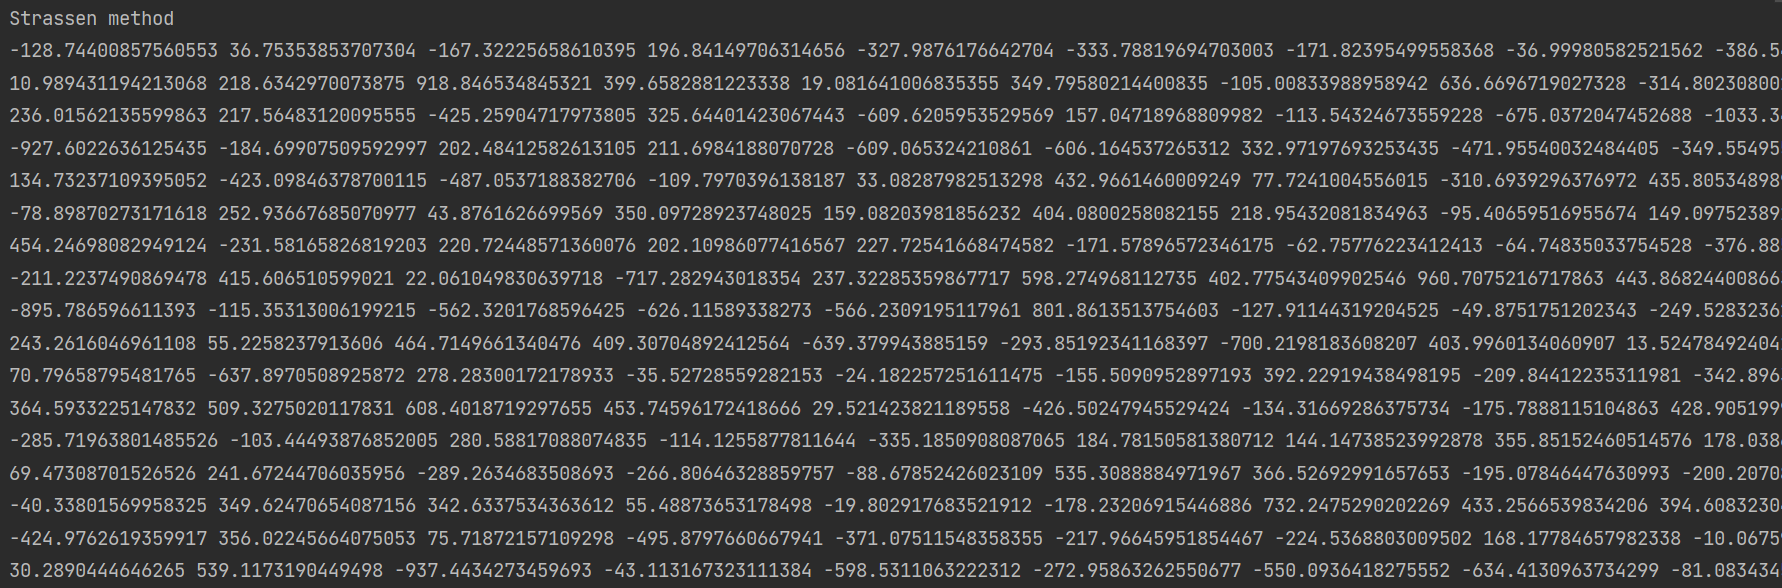
\includegraphics[width=0.8\textwidth]{img1}
\caption{Результат метода Штрассена}
\label{fig:img1}
\end{figure}

\begin{figure}[!htb]
	\centering
	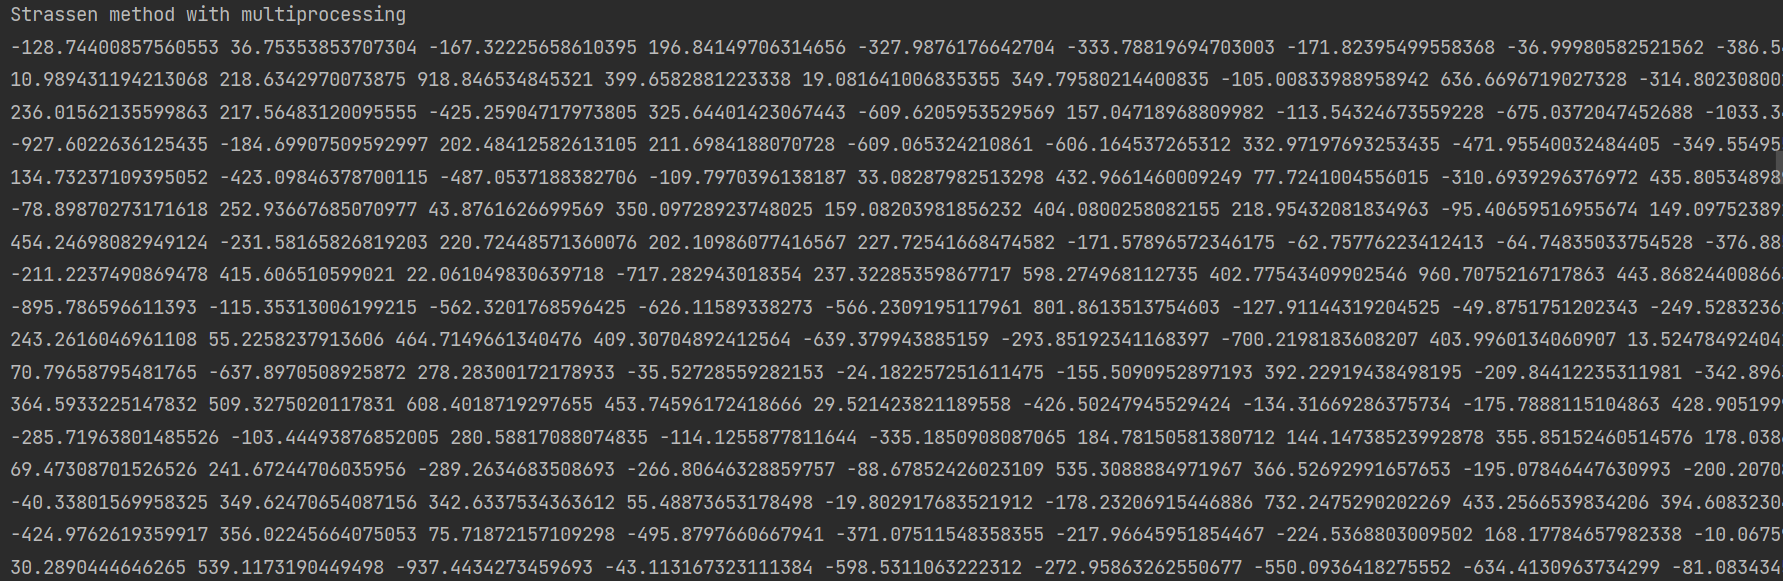
\includegraphics[width=0.8\textwidth]{img2}
\caption{Результат метода Штрассена с многопоточностью}
\label{fig:img2}
\end{figure}

\begin{figure}[!htb]
	\centering
	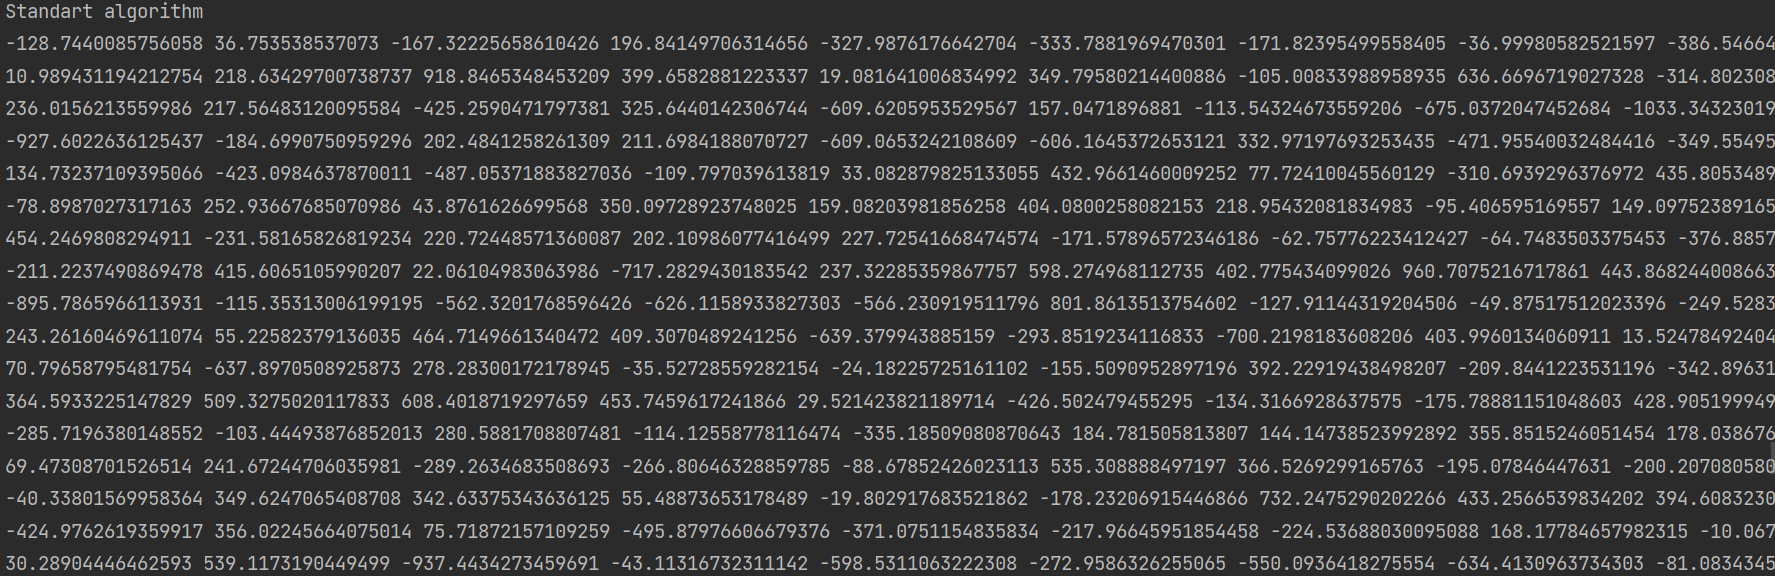
\includegraphics[width=0.8\textwidth]{img3}
\caption{Результат стандартного алгоритма}
\label{fig:img3}
\end{figure}

\begin{figure}[!htb]
	\centering
	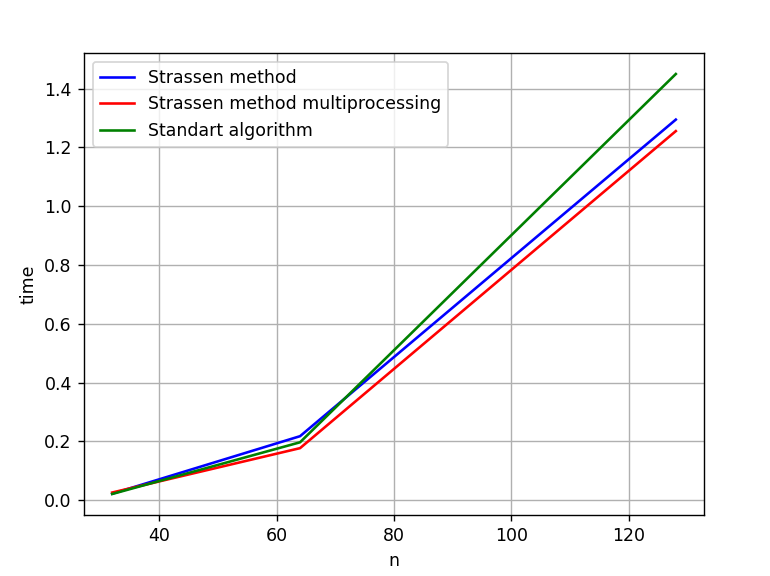
\includegraphics[width=0.8\textwidth]{img4}
\caption{График зависимости времени работы от размера матрицы}
\label{fig:img4}
\end{figure}

\begin{figure}[!htb]
	\centering
	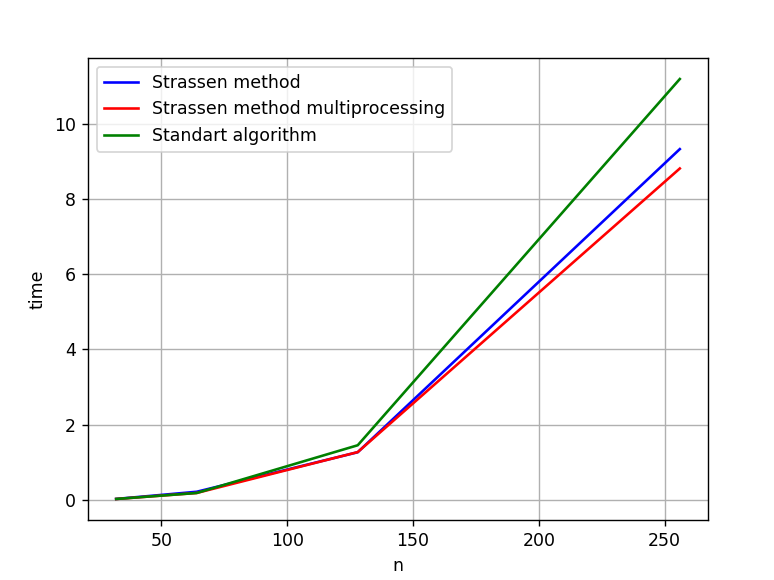
\includegraphics[width=0.8\textwidth]{img5}
\caption{График зависимости времени работы от размера матрицы}
\label{fig:img5}
\end{figure}

\section{Выводы}\label{Sect::conclusion}

В результате выполнения лабораторной работы был реализован метод Штрассена, метод Штрассена с многопоточностью, проведены сравнения времени работы со стандартным алгоритмом.

\end{document}
